\documentclass[tikz,border=8pt]{standalone}
% Shared look for every TikZ diagram. Load with % Shared look for every TikZ diagram. Load with % Shared look for every TikZ diagram. Load with \input{../../tools/tikz-style.tex}
\usepackage[T1]{fontenc}
\usepackage{lmodern}
\renewcommand{\sfdefault}{lmr}  % diagrams use the same serif as the text
\usetikzlibrary{arrows.meta, positioning, shapes.geometric, calc, fit, backgrounds}
\definecolor{cblue}{HTML}{4C78A8}
\definecolor{corange}{HTML}{F58518}
\definecolor{cgreen}{HTML}{54A24B}
\definecolor{cred}{HTML}{E45756}
\definecolor{cpurple}{HTML}{B279A2}
\definecolor{cgrey}{HTML}{6B6B6B}
\tikzset{
  every picture/.style={font=\sffamily, line width=1.2pt},
  box/.style={draw=#1, fill=#1!12, rounded corners=4pt, align=center, inner sep=7pt, minimum height=1.1cm},
  box/.default=cgrey,
  arrow/.style={-{Stealth[length=3mm]}, draw=cgrey, line width=1.4pt},
  title/.style={font=\sffamily\bfseries\Large},
  note/.style={font=\sffamily\small, text=cgrey, align=center},
}
\AtBeginDocument{\hyphenpenalty=10000 \exhyphenpenalty=10000}

\usepackage[T1]{fontenc}
\usepackage{lmodern}
\renewcommand{\sfdefault}{lmr}  % diagrams use the same serif as the text
\usetikzlibrary{arrows.meta, positioning, shapes.geometric, calc, fit, backgrounds}
\definecolor{cblue}{HTML}{4C78A8}
\definecolor{corange}{HTML}{F58518}
\definecolor{cgreen}{HTML}{54A24B}
\definecolor{cred}{HTML}{E45756}
\definecolor{cpurple}{HTML}{B279A2}
\definecolor{cgrey}{HTML}{6B6B6B}
\tikzset{
  every picture/.style={font=\sffamily, line width=1.2pt},
  box/.style={draw=#1, fill=#1!12, rounded corners=4pt, align=center, inner sep=7pt, minimum height=1.1cm},
  box/.default=cgrey,
  arrow/.style={-{Stealth[length=3mm]}, draw=cgrey, line width=1.4pt},
  title/.style={font=\sffamily\bfseries\Large},
  note/.style={font=\sffamily\small, text=cgrey, align=center},
}
\AtBeginDocument{\hyphenpenalty=10000 \exhyphenpenalty=10000}

\usepackage[T1]{fontenc}
\usepackage{lmodern}
\renewcommand{\sfdefault}{lmr}  % diagrams use the same serif as the text
\usetikzlibrary{arrows.meta, positioning, shapes.geometric, calc, fit, backgrounds}
\definecolor{cblue}{HTML}{4C78A8}
\definecolor{corange}{HTML}{F58518}
\definecolor{cgreen}{HTML}{54A24B}
\definecolor{cred}{HTML}{E45756}
\definecolor{cpurple}{HTML}{B279A2}
\definecolor{cgrey}{HTML}{6B6B6B}
\tikzset{
  every picture/.style={font=\sffamily, line width=1.2pt},
  box/.style={draw=#1, fill=#1!12, rounded corners=4pt, align=center, inner sep=7pt, minimum height=1.1cm},
  box/.default=cgrey,
  arrow/.style={-{Stealth[length=3mm]}, draw=cgrey, line width=1.4pt},
  title/.style={font=\sffamily\bfseries\Large},
  note/.style={font=\sffamily\small, text=cgrey, align=center},
}
\AtBeginDocument{\hyphenpenalty=10000 \exhyphenpenalty=10000}

\begin{document}
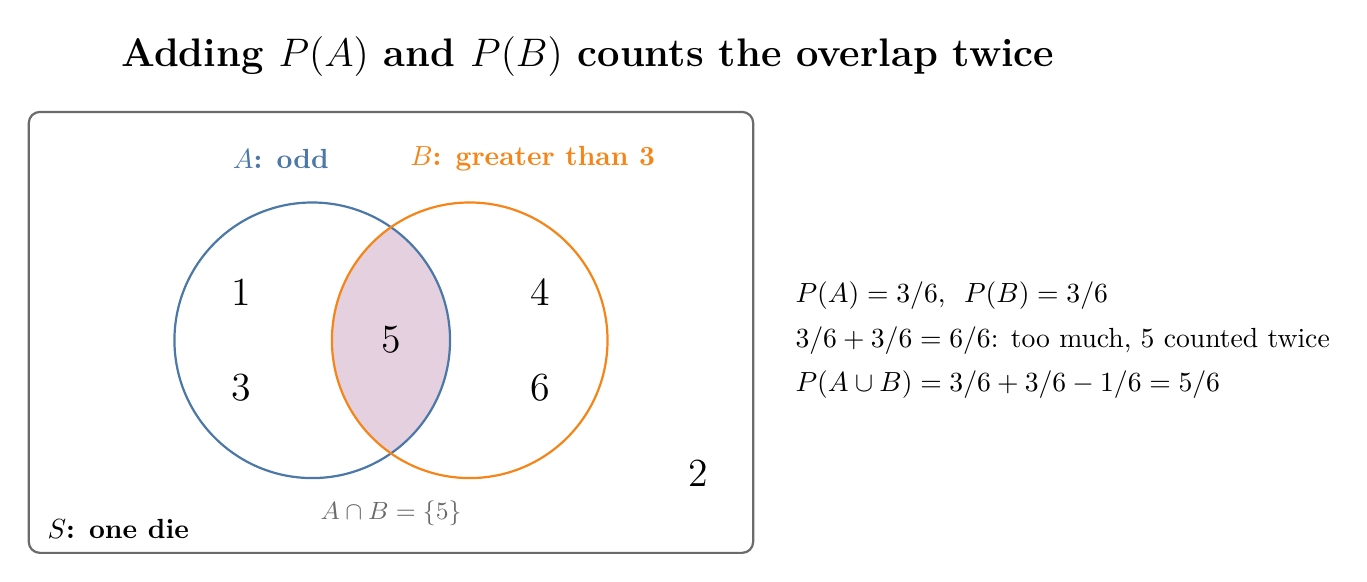
\begin{tikzpicture}[x=1cm, y=1cm]
  \node[title] at (2.5,3.6) {Adding $P(A)$ and $P(B)$ counts the overlap twice};
  \draw[thick, rounded corners, draw=cgrey] (-4.6,-2.7) rectangle (4.6,2.9);
  \node[font=\sffamily\bfseries, anchor=south west] at (-4.5,-2.65) {$S$: one die};
  \begin{scope}
    \clip (-1.0,0) circle (1.75);
    \fill[cpurple!35] (1.0,0) circle (1.75);
  \end{scope}
  \draw[thick, cblue] (-1.0,0) circle (1.75);
  \draw[thick, corange] (1.0,0) circle (1.75);
  \node[text=cblue, font=\sffamily\bfseries] at (-1.4,2.3) {$A$: odd};
  \node[text=corange, font=\sffamily\bfseries] at (1.8,2.3) {$B$: greater than 3};
  \node[font=\sffamily\Large] at (-1.9,0.6) {1};
  \node[font=\sffamily\Large] at (-1.9,-0.6) {3};
  \node[font=\sffamily\Large] at (0,0) {5};
  \node[font=\sffamily\Large] at (1.9,0.6) {4};
  \node[font=\sffamily\Large] at (1.9,-0.6) {6};
  \node[font=\sffamily\Large] at (3.9,-1.7) {2};
  \node[note] at (0,-2.2) {$A \cap B = \{5\}$};
  \node[align=left, right] at (5.0,0) {$P(A) = 3/6$, \ $P(B) = 3/6$\\[4pt]
     $3/6 + 3/6 = 6/6$: too much, 5 counted twice\\[4pt]
     $P(A \cup B) = 3/6 + 3/6 - 1/6 = 5/6$};
\end{tikzpicture}
\end{document}
